\chapter{Performed SAXSTT Reconstructions}

\section{Reconstruction of Simulated Parallel Nanostructures}
\label{sec:reconstruction_parallel}

With a chosen data set size of $35^3$ voxels,
the SAXSTT algorithm was performed on the dataset of parallel nanostructures, as mentioned in Section \ref{sec:pp_nanostructures_reconstruction}.
The initial conditions for the reconstruction were close to the true values of the simulated nanostructures.
For instance, the true orientation was $(\theta_{op} = \pi/3$ , $\varphi_{op} = \pi/3)$, while the initial guess was $(\theta_{op} = \pi/4$, $\varphi_{op} = \pi/4)$.
On the other hand, the initial intensity value was \num{e-4} compared to the true value of 0.69.
Figure \ref{fig:coefficient_comparison_AD_SYM} and \ref{fig:orientation_comparison_AD_SYM} show distributions of spherical harmonics parameters for converged SAXSTT reconstructions.
In addition to the raw data, the results include curve fitting of the distributions to Lorentzian functions.
The peak and full width at half maximum (FWHM) of the Lorentzians are listed in Table \ref{tab:curve_fitting}.
The peak values of the Lorentzians are close to the true values of the simulated nanostructures, with a FWHM in the order of \num{e-3}.
For simplicity, the preferred orientation will from now on be denoted $\theta$ and $\varphi$ instead of $\theta_{op}$ and $\varphi_{op}$, respectively.

\begin{figure}[h!]
    \centering
    \includesvg[width=1\textwidth]{../XRD_CT/Plotting/thesis_plots/SH_coeffs_0align_closecoeffs.svg}
    \caption{ The coefficients converge to a Lorentzian distribution
        around the true value when the initial conditions have the correct sign.  }
    \label{fig:coefficient_comparison_AD_SYM}
\end{figure}

\begin{figure}[h!]
    \centering
    \includesvg[width = 1\textwidth]{../XRD_CT/Plotting/thesis_plots/SH_orientation_0align_closeangles.svg}
    \caption{  The orientation parameters converge to a Lorentzian distribution
        around the true value when the initial conditions are sufficiently close to the true value.}
    \label{fig:orientation_comparison_AD_SYM}
\end{figure}


\begin{table}[h!]
    \centering
    \caption{  The peak and FWHM of the Lorentzian curve fits
        for the coefficients and orientation parameters for the reconstruction
        with good initial conditions.}
    \label{tab:curve_fitting}
    \begin{tabular}{ c c c c c c }
        \hline %\toprule
        \textbf{}      &                   & \multicolumn{2}{c}{\textbf{Automatic (AD)}} & \multicolumn{2}{c}{\textbf{Symbolic (SYM)}}                                             \\
        \textbf{}      & \textbf{Solution} & \textbf{Peak}                               & \textbf{FWHM [\num{e-3}]}                   & \textbf{Peak} & \textbf{FWHM [\num{e-3}]} \\
        \hline %\midrule
        \textbf{a0}    & 0.690             & 0.691                                       & 5.834                                       & 0.691         & 6.764                     \\
        \textbf{a2}    & 0.230             & 0.230                                       & 2.930                                       & 0.229         & 3.906                     \\
        \textbf{a4}    & 0.115             & 0.000                                       & 0.000                                       & 0.000         & 0.000                     \\
        \textbf{a6}    & 0.575             & 0.000                                       & 0.000                                       & 0.000         & 0.000                     \\
        $\bm{\theta}$  & 1.047             & 0.000                                       & 0.000                                       & 0.000                                     \\
        $\bm{\varphi}$ & 1.047             & 0.000                                       & 0.000                                       & 0.000                                     \\
        \hline %\bottomrule
    \end{tabular}
\end{table}

\clearpage

Further analysis of the different reconstruction algorithms was performed on the so-called phantom data set.
This included comparing the result of the alternative cost function EXPSIN to the result of the Spherical Harmonics cost function.
In this case, it is not possible to directly compare the anisotropic coefficients. Thus, the degree of anisotropy (DoA) was used as a metric for the nanostructure shape.

The initial EXPSIN form factor, as listed in \eqref{eq:exp_sin_squared}, was modified through trial and error, exploiting the versatility of automatic differentiation.
The final cost function expression included normalisation of the exponential term using Simpson's rule for numerical integration.
In addition, the cost function was adjusted to account for both perpendicular and parallel scattering models, as mentioned in ...%RSD: Explain somewhere
The final cost function expression can therefore be expressed as:

\begin{equation}
    \label{eq:final_exp_sin_squared}
    \bm{\widehat{R}}(\bm{r'}, \bm{q'}) = A^{2} \frac{\exp\left( \mp |B| \sin^{2}(\Theta) \right)}{\int_{0}^{\pi} \exp\left( \mp |B| \sin^{2}(\Theta) \right) \sin(\Theta) d\Theta},
\end{equation}

where $\mp$ is a sign that depends on the scattering model. For parallel scattering, $\mp = -$, while for perpendicular scattering, $\mp = +$.
This sign determines at what $\Theta$ the exponential term is at its maximum.

With the alternative cost function optimised to some degree, the different algorithms were compared.
Figure \ref{fig:phantom_reconstruction_3D} shows a 3D representation of the reconstructed Phantom data set.
The marker colour represents the degree of anisotropy, while the orientation of the nanostructures is represented by the direction of the markers.
At a glance, the results of the different algorithms were similar.
However, SYM had the most voxels with an isotropic intensity above the threshold value of 0.1. Moreover, AD had seemingly a generally higher degree of anisotropy,
while EXPSIN had a more abrupt transition between isotropic and anisotropic voxels. A voxel was in a sense determined to be either isotropic or fully anisotropic.

\begin{figure}[h!]
    \centering
    \includesvg[height = 1\textheight]{../XRD_CT/Plotting/thesis_plots/P_3D.svg}
    \caption{ 3D reconstruction of the phantom data set.
        The reconstruction has been cropped to the region of interest,
        and the degree of anisotropy has been plotted for voxels that have an isotropic intensity, meaning a0 or A, above a threshold of 0.1. }
    \label{fig:phantom_reconstruction_3D}
\end{figure}

\clearpage
A more in-depth analysis was performed on
the individual reconstruction parameters for the centremost 2D-slice, which are shown in Figure \ref{fig:phantom_reconstruction_2D} and \ref{fig:phantom_reconstruction_2D_angles}. % RSD: Describe
In regards to the isotropic intensity parameter, $a0/A$, the different algorithms showed different degree of consistency.
Compared to the "AD"-algorithm, the "SYM"-algorithm had fewer and smaller outliers from the true value of isotropic intensity, which was 1.
However, the "SYM"-algorithm performed poorly at the interface between the sample and the surroundings.
Generally, the "EXPSIN"-algorithm's estimate of isotropic intensity was lower than the true value.
Apart from the low estimate, the "EXPSIN"-algorithm behaved similarly to the "AD"-algorithm.

%RSD: Also discuss anisotropy part, but wait for the proper metric. 

\begin{figure}[h!]
    \centering
    %RSD: Possible compilation issue if changing the plots
    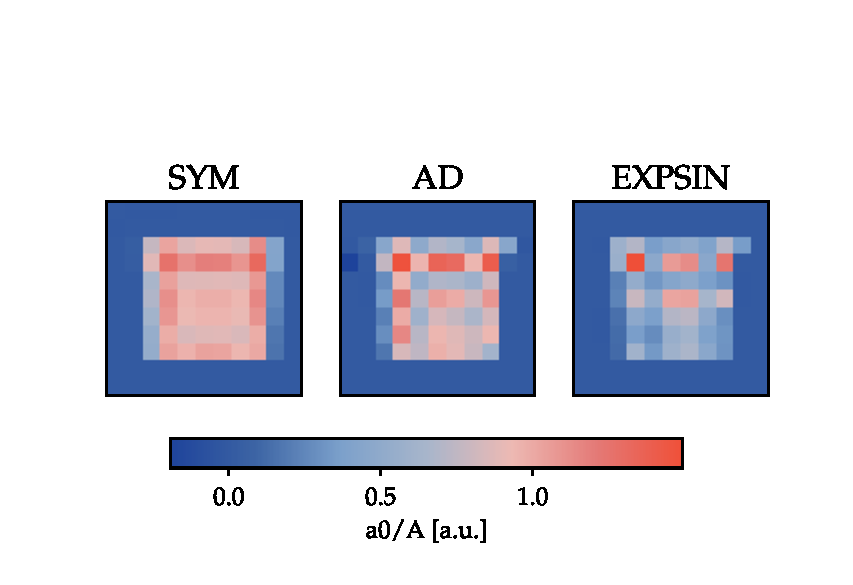
\includegraphics[trim={0 0cm 0 2.5cm},clip,width=1\textwidth]{./svg-inkscape/P_slices_A_svg-tex.pdf}
    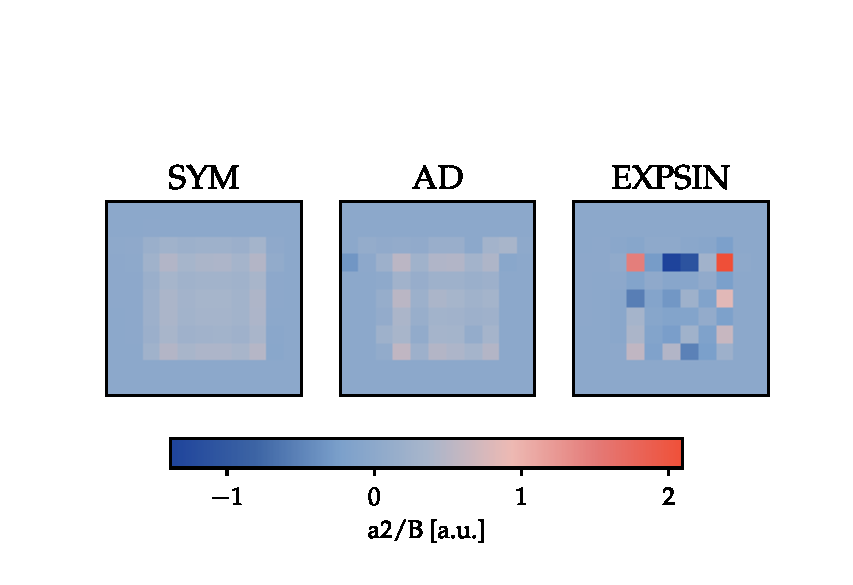
\includegraphics[trim={0 0cm 0 2.5cm},clip,width=1\textwidth]{./svg-inkscape/P_slices_B_svg-tex.pdf}
    %\adjustbox{trim = 0cm 1cm 0cm 0cm}{\includesvg[width = 1\textwidth]{../XRD_CT/Plotting/thesis_plots/P_slices_A.svg} }
    %\adjustbox{trim = 0cm 1cm 0cm 0cm}{\includesvg[width = 1\textwidth]{../XRD_CT/Plotting/thesis_plots/P_slices_B.svg} }
    %\adjustbox{trim = 0cm 0cm 0cm 3cm}{\includesvg[width = 1\textwidth]{../XRD_CT/Plotting/thesis_plots/P_slices_theta.svg}}
    %\adjustbox{trim = 0cm 0cm 0cm 3cm}{\includesvg[width = 1\textwidth]{../XRD_CT/Plotting/thesis_plots/P_slices_phi.svg}}
    \caption{ A 2D slice of the reconstructed volume that shows the isotropic parameter in the top figure, and the anisotropic parameter in the bottom figure, for the different reconstruction algorithms, respectively.
        More specifically, the slice where z = 17 is shown.}
    \label{fig:phantom_reconstruction_2D}
\end{figure}

\clearpage

Moreover, from Figure \ref{fig:phantom_reconstruction_2D_angles}, which shows the reconstructed preferred angles,
it is evident that the "EXPSIN"-algorithm had many voxels in the middle of the sample with the same set of preferred angles as the initial conditions.
In contrast, the same voxels have converged to the true value in the "AD"-algorithm and the "SYM"-algorithm, respectively,
in terms of orientation.


\begin{figure}[h!]
    \centering
    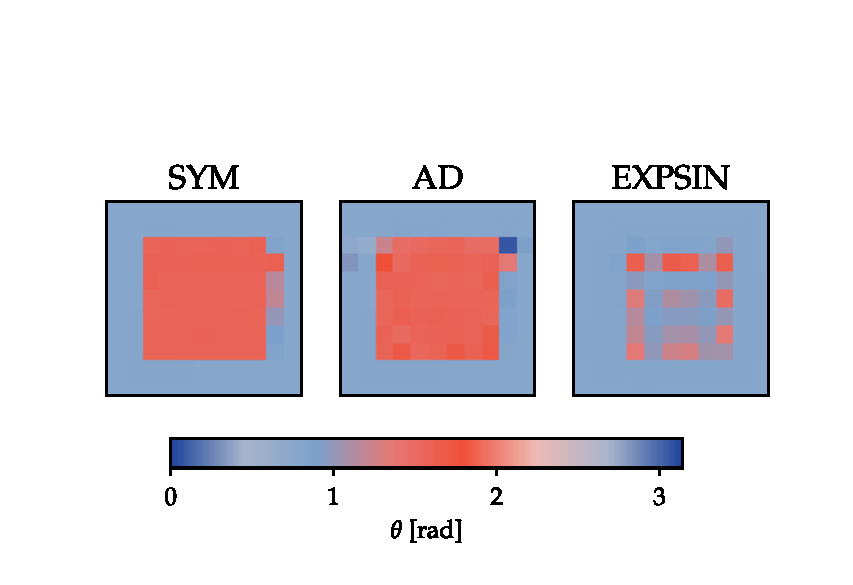
\includegraphics[trim = {0 0 0 2.5cm}, clip, width = 1\textwidth]{./svg-inkscape/P_slices_theta_svg-tex.pdf}
    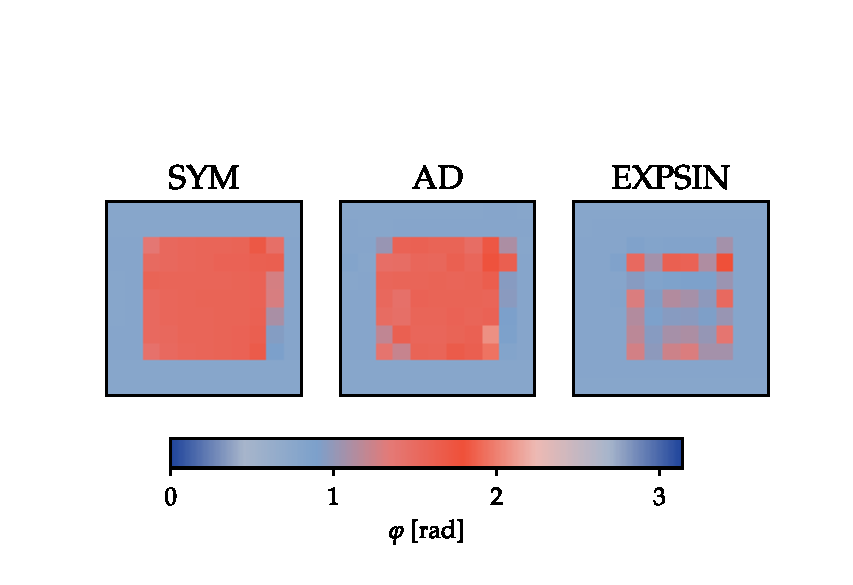
\includegraphics[trim = {0 0 0 2.5cm}, clip, width = 1\textwidth]{./svg-inkscape/P_slices_phi_svg-tex.pdf}
    \caption{ A 2D slice of the reconstructed volume that shows the preferred orientation of the reconstructed nanostructures for the different reconstruction algorithms, respectively.
        The crossection where z = 17 is shown.}
    \label{fig:phantom_reconstruction_2D_angles}
\end{figure}




\clearpage
\section{Reconstruction of Physical Carbon Knot}\label{sec:reconstruction_physical_carbon_knot}

%The general reconstruction ability of the different gradient computation methods
As a final comparison of the different SAXSTT algorithms, the reconstruction of a physical carbon knot, using actual synchrotron data, was performed.
Figure \ref{fig:carbon_knot_reconstruction_3D} shows the 3D reconstruction of the carbon knot.
Again, the marker colour represents the degree of anisotropy, while the orientation of the nanostructures is represented by the direction of the markers.
% RSD: Describe Further
All the algorithms showed similar ability to segregate the voxels containing the carbon knot from the surrounding void.
However, the "EXPSIN"-algorithm had almost twice the number of voxels with an isotropic intensity above the threshold value of 6 compared to the other algorithms.
This is an indication of a blurred interface between the carbon knot and the surrounding void.
Nevertheless, the orientation parameters seem to be correctly estimated by all the algorithms.

\clearpage

\begin{figure}[h!]
    \centering
    \includesvg[height = 1\textheight]{../XRD_CT/Plotting/thesis_plots/ck_3D.svg}
    \caption{ The resulting 3D reconstructions of the carbon knot from the "SYM"-, "AD"-, and "EXPSIN"-algorithm, respectively.
        There were 561, 533, and 900 voxels with an isotropic intensity above the threshold value of 6, respectively.
    }
    \label{fig:carbon_knot_reconstruction_3D}
\end{figure}

\clearpage

From the reconstructed volume, the centremost slice (z = 17) was investigated further.
Figure \ref{fig:carbon_knot_reconstruction_2D_coeffs} shows the isotropic coefficent, a0 or A, and the degree of anisotropy, DoA, reconstructed using symbolically, automatically, and alternatively calculated gradients, respectively.
Note that the a0 coefficient corresponds to coefficient A in the alternative cost function \eqref{eq:exp_sin_squared}.
%RSD: Describe. 
The results of the "SYM"- and "AD"-algorithm were close to indistinguishable,
while the "EXPSIN"-algorithm shared most of the same features.
However, the latter algorithm had a less pronounced edge at the interface between the sample and the surroundings.
Moreover, the amount of outliers was higher for the "EXPSIN"-algorithm.

\begin{figure}[h!]
    \centering
    \includesvg[width = 1\textwidth]{../XRD_CT/Plotting/thesis_plots/ck_slices_A.svg}
    \includesvg[width = 1\textwidth]{../XRD_CT/Plotting/thesis_plots/ck_slices_B.svg}
    \caption{  A 2D slice of the reconstructed carbon knot that shows the isotropic parameter in the top figure, and the anisotropic parameter in the bottom figure, for the different reconstruction algorithms, respectively.
        More specifically, the slice where z = 17 is shown. }
    \label{fig:carbon_knot_reconstruction_2D_coeffs}
\end{figure}

\clearpage
The determined orientations in the mentioned 2D slice are shown in Figure \ref{fig:carbon_knot_reconstruction_2D_angles}. %RSD: Describe
Again, the "EXPSIN"-result turned out to be noisy, even though the main features were reconstructed correctly.
In contrast to the isotropic and anisotropic parameters,
the "AD"-algorithm and the "SYM"-algorithm were slightly different in terms of preferred angles.
Nevertheless, the differences were small, and the edges between the sample and the surroundings were well-defined in both algorithms.

\begin{figure}[h!]
    \centering
    \includesvg[width = 1\textwidth]{../XRD_CT/Plotting/thesis_plots/ck_slices_theta.svg}
    \includesvg[width = 1\textwidth]{../XRD_CT/Plotting/thesis_plots/ck_slices_phi.svg}
    \caption{  The reconstructed preferred orientation of the carbon knot in the z=17 crossection for the different reconstruction algorithms, respectively. }
    \label{fig:carbon_knot_reconstruction_2D_angles}
\end{figure}




